\section{Experiments}
In order to validate our approach, we carry out an extensive and in depth experimental evaluation.  We study our proposed approach from three different perspectives: 

\begin{enumerate}
\item time-accuracy trade-off
\item stage-wise analysis
\item noise analysis
\end{enumerate}

We shall start by discussing time-accuracy trade-off. This allows us to study end-to-end performance of pipeline while trading off computational time.  We also do stage-wise analysis where each stage is evaluated independently of other. This helps us understand which stage is acting as bottleneck in terms of performance. Additionally, we also do noise analysis to understand the robustness of system to noise.

\subsection{Time-accuracy trade-off experiment}
In time-accuracy trade off experiment, we study how the data can be processed in less time by compromising performance. We vary certain control parameters (stage 1 threshold in this case) and observe the time it takes to process the data along with the performance of the complete pipeline. Figure \ref{fig:time-acc-tradeoff-ar-mog} shows time-accuracy trade off for varying activity ratios (AR). The trade off curve depicts f1 score on y-axis and normalized processing time on the x-axis. Next we give the definition of normalized processing time. 
$$\text{normalized time} = \frac{\text{total time to process video data}}{\text{length of video data}}$$
It is clear that as the f1 score goes up, the normalized processing time also goes up, indicating the trade off. Further, notice that the trade off curve shifts to the left as AR decreases. This is expected as stage 1 filters more and more frames with increasing threshold and thus lesser frames are processed by stage 2.The synthetic dataset parameters using in this experiment are shown in table \ref{table:fig1_data_params}. 

\begin{figure}
    \centering
    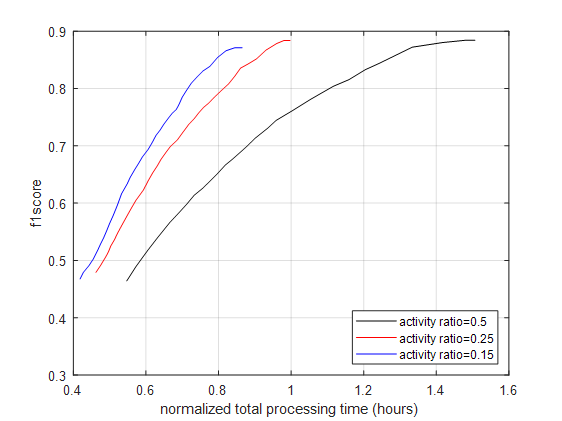
\includegraphics[width=\linewidth]{images/time-acc-tradeoff-ar-mog.png}
    \caption{Time-accuracy trade off for varying AR}
    \label{fig:time-acc-tradeoff-ar-mog}
\end{figure}

\begin{table}
\centering
\caption{Synthetic data parameters for time-accuracy trade off} \vspace{5pt}
\label{table:fig1_data_params}
\begin{tabular}{|l|l|}
\hline
parameter             & value  \\ \hline \hline
p                     & 1\%    \\ 
$\mu$    & 0.50\% \\ 
$\sigma$ & 0.20\% \\ \hline
\end{tabular}
\end{table}

\subsection{Stage-wise analysis experiments}
In this part, we analyse both stage 1 and 2 independently. We use AUC (Area Under the Curve) as the evaluation metric since it is not affected by class imbalance. We naturally have class imbalance since very few trespassing frames exist as compared to other frames. Table \ref{table:auc-time-analysis-s1} shows that stage 1 takes only 30 ms where as stage 2 takes around 500 ms on $1080 \times 960$ sized frame. This shows that stage 1 is approx. $16.7$ times faster than stage 2 wich resonates with our goal stated in Section \ref{sec:goal}. 

\textcolor{red}{stage 2 methodoloy-if space permits}

\begin{table}
\centering
\caption{Stage 1 AUC and time analysis} \vspace{5pt}
\label{table:auc-time-analysis-s1}
\begin{tabular}{|l|l|c|}
\hline
stage   	& AUC     & mean processing \\
            &         &  time (ms)  \\ \hline \hline
stage 1     & 0.94    & 30    \\
stage 2     & 0.81    & 500  \\ \hline
\end{tabular}
\end{table}


\subsection{Noise analysis experiments}
Third and final part of our experimental evaluation is noise analysis. In this part, we evaluate the robustness of stage 1 against noise. In terms of noise, we have 3 parameters: $p, \mu, \text{ and } \sigma$. Description of these parameters has been discussed in table \ref{table:noise-params}. To study the influence of one parameter, we vary it while keeping the others constant. 

Table \ref{table:noise-analysis-auc-mog} shows AUC for stage 1 varying $p$ and $\mu$. We use the noise parameters ($AR=0.5$, $\mu=0.5\%$, $\sigma=0.2\%$) while varying $p$ and ($AR=0.5$, $p=2\%$, $\sigma=0.2\%$) while varying $\mu$. For both $p$ and $\mu$, it is clear that increase in noise level decreases the performance of stage 1.  


\begin{table}
\centering
\caption{Noise analysis - AUC for varying $p$ and $\mu$} \vspace{5pt}
\label{table:noise-analysis-auc-mog}

\begin{tabular}{l r}

\begin{tabular}{|l|l|}
\hline
$p$         & AUC  \\ \hline \hline
2\%         & 0.93   \\
4\%         & 0.87    \\ 
6\%         & 0.83      \\ 
8\%         & 0.78       \\ \hline
\end{tabular}


\begin{tabular}{|l|l|}
\hline
$\mu$         & AUC  \\ \hline \hline
0.5\%         & 0.93   \\
0.7\%         & 0.92    \\ 
0.9\%         & 0.91      \\ 
1.1\%         & 0.88       \\ \hline
\end{tabular}

\end{tabular}

\end{table}
